

\section{Subsampling}

To analyze the data, the assumption of IID-ness will be needed, but without further modification the samples do not uphold it.
For instance, if a process finishes with a large turnaround time, which is caused by a long queue, it is likely that the same thing will happen for the next processes.

To address this and ensure independence between samples, subsampling has been employed. The new sample is constructed taking each point of the starting sample with probability $p$.
$p = \frac{1}{2^k}$ and $k$ is the smallest integer that passes the Ljung-Box test.
Using the Ljung-Box test makes it possible to automate the subsampling step. It was implemented to test the first 30 lags, with a significance level of 5\%, with these values the sample is considered independent if:
\vspace{-0.5\baselineskip}
\begin{equation}
    Q = n(n+2) \sum_{k=1}^{30} \frac{\hat{\rho}_k^2}{n-k} < \chi^2_{0.95,30} \approx 43.77
\end{equation}
As utilization increases, the correlation becomes stronger, as shown in \cref{fig:autoCorComparison}.

% todo dare nomi ai grafici con metrica che ti dice quanto saturo (bello se definita nella parte iniziale)
\begin{figure}[H]
    \captionsetup{type=figure}
    \centering
    \begin{subfigure}[b]{0.45\textwidth}
        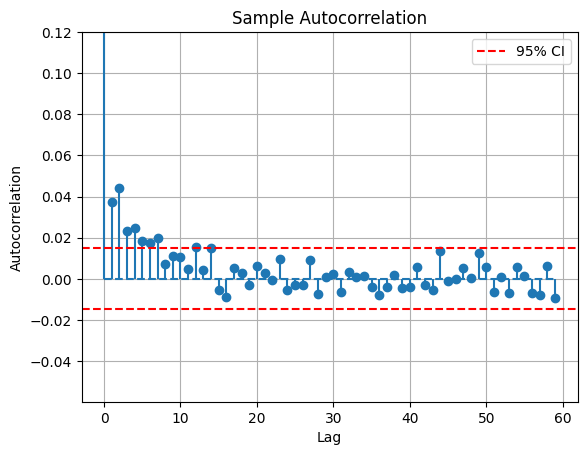
\includegraphics[width=\textwidth]{./images/04/autoCor/autoCorLowUnfix.png}
        \caption{$\rho=0.4$, Q = 119}
        \label{fig:autoCorLowUnfix}
    \end{subfigure}
    \hfill % Add space between the subfigures
    \begin{subfigure}[b]{0.45\textwidth}
        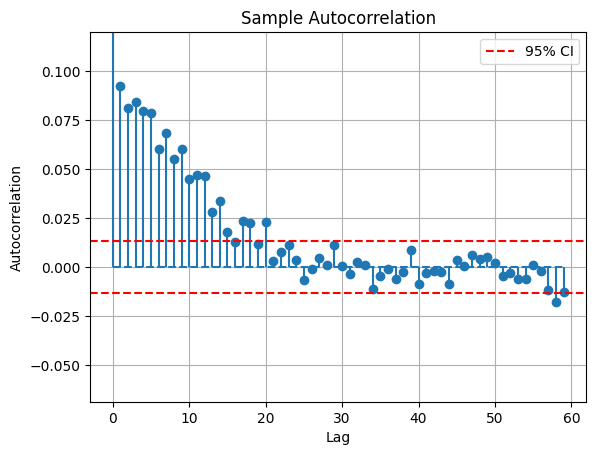
\includegraphics[width=\textwidth]{./images/04/autoCor/autoCorHighUnfix.png}
        \caption{$\rho=0.5$, Q = 1333}
        \label{fig:autoCorHighUnfix}
    \end{subfigure}
    \vspace{15pt} % Add vertical space between the two rows

    \begin{subfigure}[b]{0.45\textwidth}
        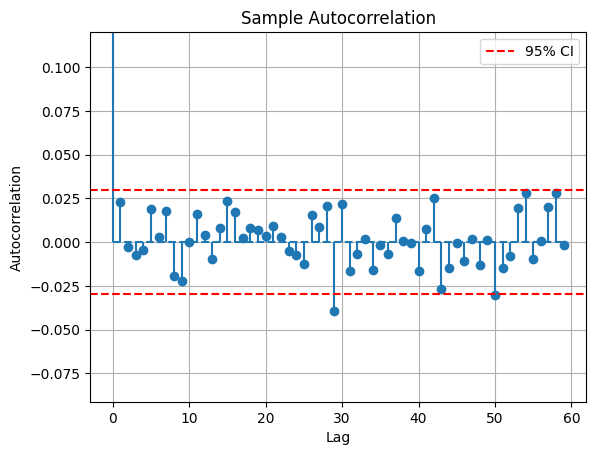
\includegraphics[width=\textwidth]{./images/04/autoCor/autoCorLowFix.png}
        \caption{$\rho=0.4$, $p=1/4$, Q = 27}
        \label{fig:autoCorLowFix}
    \end{subfigure}
    \hfill % Add space between the subfigures
    \begin{subfigure}[b]{0.45\textwidth}
        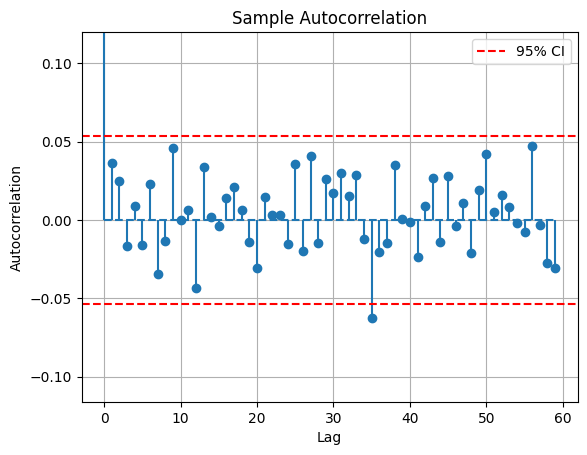
\includegraphics[width=\textwidth]{./images/04/autoCor/autoCorHighFix.png}
        \caption{$\rho=0.5$, $p=1/16$, Q = 22}
        \label{fig:autoCorHighFix}
    \end{subfigure}
    \vspace{10pt} % Add vertical space before the caption
    \caption{Comparison of turnaround time autocorrelation with and without subsampling for different loads.}
    \label{fig:autoCorComparison}
\end{figure}
